\documentclass[conference]{IEEEtran}
\IEEEoverridecommandlockouts
\usepackage{cite}
\usepackage{amsmath,amssymb,amsfonts,amsthm}
\usepackage{graphicx}
\usepackage{booktabs}
\usepackage{multirow}
\usepackage{xcolor}
\usepackage{url}
\newtheorem{proposition}{Proposition}

\begin{document}

\title{Order-Independent Face Grouping with Persistent User Corrections:\\ A Simulation Study for Local-First Photo Libraries}

% AUTHORS: replace the bracketed fields with the real details before submission (do NOT submit placeholders).
\author{\IEEEauthorblockN{Anugrah Singh}
\IEEEauthorblockA{\textit{Dept. of Computer Science and Engineering} \\
\textit{[College name]}\\
[City], India \\
[email]}
\and
\IEEEauthorblockN{Yadriksha Uprety}
\IEEEauthorblockA{\textit{Dept. of Computer Science and Engineering} \\
\textit{[College name]}\\
[City], India \\
[email]}
}

\maketitle

\begin{abstract}
Photo managers that group faces on the user's own device must update the groups as photos arrive, and users correct them
by hand. Greedy incremental clustering makes the people found depend on import order, and re-clustering from scratch
undoes the corrections. We study the face clusterer of Cove, a local-first photo manager, whose output is a function of the
set of faces and the set of must-link and cannot-link corrections: single linkage over core faces, an attach step and a
centroid merge. On simulated libraries whose people are disjoint from the tuning data, its accuracy without corrections is
within about one point of average linkage overall (ahead on clean photos, behind on low-resolution photos and, by 7 points,
on profile ones), and on web family photos (FIW) with no retuning it again ties average linkage. With corrections (three
simulated users, EdgeFace-S) it is within 0.003 F1 of constrained average linkage. It keeps every consistent correction
across the next import, where plain re-clustering keeps 20\% and re-applying keeps 73--96\%, and its read step is roughly an
order of magnitude faster than constrained average linkage on synthetic libraries of up to 50{,}000 faces. Recomputing from
the two sets, as any such design would, gives in simulation identical people on two devices (53\% and 31\% for a
frozen-label rule of our design), exact retraction and deletion, and corrections that keep about half their gain under a
different recogniser. For our clusterer the gain from corrections is gone by about one wrong click in twenty, while
re-applying and constrained average linkage degrade more gently, so a review-and-undo view is advisable. Only the clusterer
is in the application; corrections, devices and users are simulated.
\end{abstract}

\begin{IEEEkeywords}
face clustering, constrained clustering, incremental clustering, user corrections, local-first software, photo libraries
\end{IEEEkeywords}

% ---------------------------------------------------------------------------------------------------------------------
\section{Introduction}
People most often search a personal photo collection by person. Self-hosted, local-first managers such as
Immich~\cite{immich}, PhotoPrism~\cite{photoprism}, FaceCluster~\cite{filonenko2025facecluster} and the Cove system
studied here group faces on hardware the user controls. On such a device the library is never complete: photos arrive in
batches, and users merge and split people by hand. Two problems follow that a one-off benchmark does not show:
(1) \textbf{order dependence}: the cheapest update is a greedy \emph{leader} pass~\cite{hartigan1975clustering}, whose
result depends on import order; and (2) \textbf{lost corrections}: re-clustering from scratch does not take the user's
earlier fixes as input, so the same mistakes return.

Constrained clustering~\cite{wagstaff2001copkmeans,davidson2005agglomerative}, its incremental
form~\cite{davidson2007incremental}, axioms for incremental clustering~\cite{bandyopadhyay2016axioms} and
interactive face annotation~\cite{tian2007face,cui2007easyalbum} are established, and we claim none of them. This is an
application-and-measurement study. Its contributions are:
\begin{itemize}
\item a clusterer from known parts whose output, including corrections, does not depend (up to exact ties) on the order or batching of
insertions or on deletions, with a short argument and an exact, faster read step (Sec.~\ref{sec:method});
\item a comparison of four ways to keep corrections when photos arrive, with three simulated users and a sweep of the
error rate (Sec.~\ref{sec:corr}), and of what recomputing from the sets buys, against a frozen-label baseline we designed
(Sec.~\ref{sec:conseq});
\item an identity-disjoint accuracy evaluation with fairer tuning that reports where our method is worse (Sec.~\ref{sec:acc}),
an outside test on web family photos (FIW), and a scale test to 50{,}000 faces (Sec.~\ref{sec:time}).
\end{itemize}
Only the clusterer is part of the application; the corrections, devices and users in the evaluation are simulated from public
benchmarks. Code and per-run results are released.

% ---------------------------------------------------------------------------------------------------------------------
\section{Related Work}
\textbf{Face clustering.} Large-scale methods use approximate rank-order distances~\cite{otto2018clustering} or graph
networks trained on labelled clusters~\cite{wang2019linkage,yang2019affinity}. We compare with training-free methods a CPU
application can run: leader clustering, single and average linkage, DBSCAN~\cite{ester1996dbscan} and
HDBSCAN~\cite{campello2013hdbscan}.

\textbf{Incremental and constrained clustering.} Incremental DBSCAN~\cite{ester1998incremental} gives the result of
re-running DBSCAN after each insertion or deletion, up to border points; our core-point step builds on it, and we add corrections
and the centroid merge. Must-link and cannot-link constraints were brought to $k$-means~\cite{wagstaff2001copkmeans} and
agglomerative clustering~\cite{davidson2005agglomerative}, to density-based clustering~\cite{ruiz2007cdbscan} (our constrained
step is closest to C-DBSCAN), to faces~\cite{shi2018conpac,wu2013constrained} and to incremental
settings~\cite{davidson2007incremental,monath2019grinch}. Constraint sets can lower accuracy~\cite{davidson2006utility}, imperfect
users need special handling~\cite{zhu2016imperfect,mazumdar2017noisy}, and OGMC~\cite{montero2022ogmc} reduces order dependence
for face streams.

\textbf{Sets, replicas and upgrades.} Computing state from the set of inputs so that replicas that exchange inputs agree is
the idea of conflict-free replicated data types~\cite{shapiro2011crdt} and local-first software~\cite{kleppmann2019local}.
Splitting a linkage clustering at the components of a threshold graph is classical for single
linkage~\cite{gower1969mst,sibson1973slink}. Backward-compatible embeddings~\cite{shen2020backward} address upgrades for the
embeddings themselves. In sources searched on 2026-11-10 (SciSpace, Consensus, web search, mostly abstracts) we did not find a
measurement of whether face-grouping corrections survive re-clustering, agree across devices, can be retracted exactly, or
survive a change of recogniser; this is bounded to those sources.

% ---------------------------------------------------------------------------------------------------------------------
\section{Method}\label{sec:method}
\begin{figure}[t]
\centering
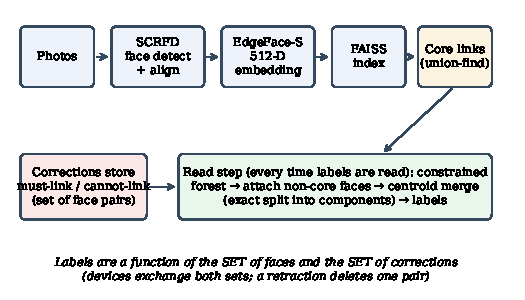
\includegraphics[width=0.92\columnwidth]{figs/pipeline.pdf}
\caption{The pipeline. Corrections are kept as a set of face pairs next to the face index; the read step is recomputed from
both sets, so devices that exchange the two sets, or a deletion of one pair, give the same result as starting again (simulated; the
application has no sync).}
\label{fig:pipeline}
\end{figure}
\textbf{Pipeline} (Fig.~\ref{fig:pipeline}). Faces are detected with SCRFD-500M~\cite{guo2022scrfd}, aligned to $112\times112$
and embedded with EdgeFace-S~\cite{george2024edgeface} (MobileFaceNet \texttt{w600k\_mbf}, ``MBF'', is also evaluated); unit vectors give
cosine similarity $s(i,j)$ and go into a FAISS flat index~\cite{johnson2021faiss}.

\textbf{Clusterer.} Fix thresholds $\tau_\ell\ge\tau_a$, a neighbour count $m$ and a merge threshold $\tau_g$. Face $i$ is
\emph{core} if at least $m$ other faces have $s\ge\tau_\ell$; core faces with $s\ge\tau_\ell$ are linked, and clusters are
the components of the link graph. A non-core face joins its most similar core face if $s\ge\tau_a$, else stays alone.
Cluster centroids are then merged by average linkage at similarity $\tau_g$. At the tuned $m=1$ the core step is single
linkage at $\tau_\ell$, so the method is single linkage, plus attachment, plus a centroid merge; Sec.~\ref{sec:acc} measures each part.

\textbf{Incremental update.} A new batch needs one FAISS range search at $\tau_a$; neighbour lists are extended, faces whose neighbour
count reaches $m$ become core, and new core faces are unioned with their core neighbours. Core status and links only switch from
false to true; attachment and the merge are recomputed when labels are read.

\textbf{Exact read step.} Here average linkage treats each cluster centroid as one item, and the similarity of two groups of
centroids is the mean of their pairwise centroid cosines. That mean cannot exceed its largest term, so two groups never join
unless some cross pair has cosine $\ge\tau_g$. We therefore split the centroids into components of the graph of pairs with
cosine $\ge\tau_g$ and agglomerate each alone. The split is classical for single linkage; for this average linkage it follows from
the argument above, and we use it for speed. It gave identical partitions to the original merge on all 240 test library--condition
pairs, for both recognisers, under the corrections of three simulated user models (a separate run from Sec.~\ref{sec:corr}: 210--216 pairs per user
received corrections, which changed the result in all but one of 1{,}276 cases) and on 8{,}290 faces (Sec.~\ref{sec:time}).

\textbf{Corrections and deletion.} A user states that faces $i,j$ are the same person (must-link) or different people
(cannot-link). Both are stored as sets of face pairs and applied whenever labels are computed. In order: (1) must-links, in
decreasing cosine of the pair (ties by the faces' content, not their ids), each joining two groups unless that would put a
cannot-linked pair into one group; (2) core links, in decreasing similarity (ties by face id), under the same test; (3) each non-core face
whose group has no core face attaches to its most similar allowed core face; (4) the centroid merge never joins clusters
holding a cannot-linked pair. A cannot-link is therefore never violated, and in a conflict ($a{=}b$, $b{=}c$, $a{\ne}c$) the
less similar must-link is the one dropped. Two non-core faces joined by a must-link attach separately, so the must-link
can join the two clusters they attach to. With corrections the read step recomputes steps (1)--(4) from scratch. Deleting photos removes the faces from the face set, drops corrections that name
them, recomputes core flags from the stored neighbour lists and rebuilds the union-find, with no new similarity search. Corrections
refer to faces by id; an application must key them by photo hash and face box so that they survive deletions and can be exchanged
between devices.

\begin{proposition}
For fixed thresholds, the labels after any sequence of insertions and deletions depend only on the final set of faces and
the corrections that name them, not on the order, batching or deletion history (in exact arithmetic, up to renaming of clusters and to exact
ties between similarities, including ties at a threshold).
\end{proposition}
\begin{proof}[Proof sketch]
Each pair of present faces with $s\ge\tau_a$ is found once, when its later face arrives; deletion removes exactly the
entries that name deleted faces. So the neighbour lists are those of the final set. Core flags are functions of these lists
and are recomputed after a deletion. In steps (1)--(3) every union is decided by the neighbour lists and a total order on
pairs by similarity, so the groups depend only on the lists and on the corrections; attachment and the centroid merge are
deterministic functions of the groups. Core-link ties are broken by face id, which depends on insertion order, so the statement
holds up to exact ties; none changed a result in our runs (order agreement 1.000 in every order tested), and a unit test checks
that deleting faces gives the same labels as never having added them.
\end{proof}
% ---------------------------------------------------------------------------------------------------------------------
\section{Experimental Protocol}\label{sec:protocol}
The main protocol was fixed before any test number was computed; the later checks (finer grids, identity bootstrap,
error-rate sweep, scale and deletion tests, FIW) are reported as additions.

\textbf{Libraries.} LFW~\cite{huang2007lfw} identities are split once (seed 2026) into a tuning and a test half, for ``family''
identities ($\ge$10 photos; 79 per half) and ``strangers'' (1{,}844 per half). A library draws 15--40 family people (up to 200
photos each) and 50--150 strangers (one photo each) from one half: 30 tuning and 30 test libraries, no person shared.
\emph{Look-alike} libraries add the 7--14 test people most similar to one person. CALFW~\cite{zheng2017calfw} (age) and
CPLFW~\cite{zheng2018cplfw} (pose) are clustered whole on test identities (8{,}212 and 7{,}718 faces). Photos are re-embedded
after degradation (low-res, blur, JPEG, dark, occluded, mixed).
\emph{Web family photos:} FIW~\cite{robinson2016fiw,robinson2018fiw} has 34{,}692 face crops of 5{,}773 people in 980 families. We split
the families into two halves (no relatives shared), build 20 tuning and 30 test libraries of 8--16 families, and use the same
detector (no face was found in 2{,}320 crops, which were resized instead of dropped), recogniser, methods and metrics. FIW is used
under its terms (non-commercial research, images not redistributed).

\textbf{Tuning.} Every method gets a grid over the same similarity range (0.20--0.70, step 0.05) and is tuned on the
same tuning libraries and conditions to maximise the adjusted Rand index (ARI)~\cite{hubert1985ari}; we report B-Cubed F1. The recogniser (EdgeFace-S) was
chosen on tuning data by a pre-declared rule.
Tuned: $\tau_\ell=0.65$, $m=1$, $\tau_a=0.50$, $\tau_g=0.55$. The terms are equal in data and rule, not in
freedom: ours has four parameters (360 grid points), one-threshold baselines one (11). Sec.~\ref{sec:acc} repeats the
comparison with finer baseline grids and with a small budget for ours.

\textbf{Test.} On the LFW libraries every method runs in 5 shuffled orders (on FIW, order-dependent methods 5, the others 3). We report B-Cubed~\cite{bagga1998entity,amigo2009bcubed} and
the \emph{order agreement} (lowest ARI between two orders). Differences use a paired bootstrap over libraries (over
library--condition pairs for corrections; 10{,}000 resamples, 95\% intervals); for Table~\ref{tab:acc} we also resample
\emph{people} (Poisson(1) weights on the 1{,}571 distinct identities in the test libraries, 1{,}000 resamples), which keeps the people shared by libraries shared.

\textbf{Corrections.} Each test library is split into ``now'' (80\%) and ``later'' (20\%). A simulated user makes up to ten
corrections on the ``now'' clustering, one at a time, aimed at the largest remaining mistake. The \emph{precise} user picks
the central face of the main person and the most similar face of the other; the \emph{casual} user picks random faces of the
two people; the \emph{error-prone} user is casual, but with probability 0.1 each correction is a wrong ``same person''
between look-alike clusters. After the ``later'' photos arrive we compare: \emph{ours}; \emph{constrained average
linkage} (our implementation after~\cite{davidson2005agglomerative}); \emph{re-apply} (cluster without corrections, then
repair each violated pair); and \emph{frozen} (earlier people kept, each new face joins its most similar face's person at
cosine $\ge0.5$, Immich's default threshold~\cite{immich}). We report F1 and the share of corrections still true. No parameter is tuned here.
\emph{Error rate}: the casual user with wrong-click probability $p\in\{0,0.02,0.05,0.1,0.2\}$.
\emph{Two devices}: a synced 50\% base, then 25\% more faces per device in its own order and up to five precise corrections,
then an exchange of faces and corrections. \emph{Retraction}: for libraries where the error-prone user made a wrong ``same
person'', retract the first after the ``later'' photos arrive. \emph{Upgrade}: the 210 libraries whose faces are identical
under both recognisers, corrections made under one and clustering run with the other. In the last three the alternative is
a frozen-label store whose corrections are label edits and whose second device replays the other's edits in received order.
This baseline is our own design, not any product's sync.

% ---------------------------------------------------------------------------------------------------------------------
\section{Results}
\subsection{Order dependence and accuracy without corrections}\label{sec:acc}
First-Leader reaches an order agreement of 0.56 and its F1 differs by up to 5.9 points between orders; adding a centroid
merge (Two-stage) still reaches 0.76 (Table~\ref{tab:acc}). Ours gave identical partitions in every order and batch split.
Single and average linkage are also invariant, and DBSCAN nearly so, but these batch methods are re-run on the whole library
after each import.

\begin{table*}[t]
\caption{B-Cubed F1 on identity-disjoint test data, EdgeFace-S embeddings (mean over 30 libraries; whole test-half sets
for CALFW/CPLFW; FIW: 30 libraries of web family photos with the LFW-tuned settings, no retuning; four methods are within 0.004). Every method tuned on the same grid range and tuning libraries. First-Leader: greedy leader pass; Two-stage: leader pass plus centroid merge; no attach: ours with $\tau_a=\tau_\ell$. JPEG (q8) row omitted (0.993 for ours and average linkage). Bold: best. Last row: lowest order
agreement (ARI between two orders) over all library conditions.}
\label{tab:acc}
\centering\small
\setlength{\tabcolsep}{5pt}
\begin{tabular}{lcccccccc}
\toprule
Condition & First-Leader & Two-stage & Single link. & DBSCAN & HDBSCAN & Avg.\ linkage & Ours, no attach & \textbf{Ours} \\
\midrule
Clean      & 0.992 & 0.985 & 0.994 & 0.994 & 0.996 & 0.992 & 0.987 & \textbf{0.998} \\
Blur       & 0.980 & 0.991 & 0.986 & 0.986 & 0.995 & 0.993 & 0.990 & \textbf{0.997} \\
Dark       & 0.989 & 0.993 & 0.993 & 0.993 & 0.993 & 0.995 & 0.988 & \textbf{0.997} \\
Low-res    & 0.917 & \textbf{0.986} & 0.963 & 0.958 & 0.975 & \textbf{0.986} & 0.978 & 0.980 \\
Mixed      & 0.902 & \textbf{0.981} & 0.956 & 0.955 & 0.948 & \textbf{0.981} & 0.978 & 0.978 \\
Occluded   & 0.852 & \textbf{0.952} & 0.800 & 0.805 & 0.925 & \textbf{0.952} & 0.907 & 0.943 \\
CALFW (age)  & 0.681 & 0.902 & 0.945 & 0.793 & 0.358 & 0.940 & 0.919 & \textbf{0.947} \\
CPLFW (pose) & 0.600 & 0.897 & 0.846 & 0.516 & 0.520 & \textbf{0.909} & 0.892 & 0.841 \\
FIW (family photos) & 0.755 & 0.782 & 0.774 & 0.745 & 0.729 & 0.785 & 0.783 & 0.786 \\
\midrule
Order agreement (min) & 0.562 & 0.758 & 1.000 & 0.997 & 0.983 & 1.000 & 1.000 & 1.000 \\
\bottomrule
\end{tabular}
\end{table*}

Our method is not clearly ahead on degraded photos. \emph{Fairer tuning.} Re-tuning every baseline on a step-0.01 grid
(581 configurations) did not help them (average linkage 0.9849 against 0.9857; none moved by more than 0.0021), and giving
ours only 51 random grid points scores 0.9809 to 0.9857 (mean 0.9836) against 0.9854. Resampling people
instead of libraries widens the intervals (eight library conditions; no multiplicity correction). Against average linkage, the strongest baseline, ours is better on clean
($+0.0059$, $[+0.0020,+0.0119]$), blur ($+0.0038$) and dark photos ($+0.0022$), worse on low-res ($-0.0061$,
$[-0.0139,-0.0008]$), and not distinguishable on JPEG (0.993 for both), mixed ($-0.0025$, $[-0.0060,+0.0002]$), occluded ($-0.0089$,
$[-0.0219,+0.0072]$) and look-alike libraries. Against single linkage ours is better on every condition by 0.2 to 14 points,
except CPLFW, where it is 0.5 points worse (0.841 vs.\ 0.846); the gain is the attach threshold, whose removal costs up to
3.6 points on libraries but gains about 5 on CPLFW. With MBF the pattern is similar, but on occluded faces ours is worse (0.928
against 0.954).

On whole sets ours trades recall for precision: best on CALFW (0.947), about 7 points below average linkage on CPLFW (0.841 vs.\
0.909; precision 0.985 vs.\ 0.912, recall 0.733 vs.\ 0.906), because single-linkage cores split profile photos from frontal
ones.

\emph{Web family photos (FIW).} On FIW we changed nothing (Table~\ref{tab:acc}). Ours scores 0.786, tied with average linkage (0.785;
difference $+0.0006$, $[-0.0046,+0.0061]$) and above single linkage ($+0.011$), DBSCAN ($+0.040$), HDBSCAN ($+0.057$) and
First-Leader ($+0.031$), whose order agreement is 0.64 against 1.000 for ours; the DBSCAN and HDBSCAN gaps are $+0.011$ and
$+0.016$ when every method is re-tuned on the tuning families, which also leaves ours tied with average linkage (0.785 against
0.788, $-0.0024$, $[-0.0082,+0.0036]$). Without the attach step ours scores 0.783. MobileFaceNet agrees (ours 0.783, average linkage 0.782; re-tuned
$-0.0042$, $[-0.0092,+0.0010]$). The 30 libraries share families, so the intervals are probably
too narrow. Scores are far below LFW's, probably because the faces are small (6.7\% were resized, not aligned) and relatives look alike.

\subsection{Keeping corrections when new photos arrive}\label{sec:corr}
For the precise user, 207 of 240 library--condition pairs needed a correction (6.3 on average among them, 5.4 over all).
They raised F1 on the ``now'' photos from 0.984 to 0.994 (gain $+0.010$, $[+0.008,+0.011]$). Table~\ref{tab:corr} shows
what happens after the ``later'' photos arrive: plain re-clustering keeps 20\% of the corrections and F1 falls back to
0.985. Ours keeps every consistent correction by construction, so the informative comparison is with other ways of keeping them.

\emph{Constrained average linkage} also keeps every correction at similar accuracy: ours is $+0.001$ F1 on all faces
($[-0.000,+0.002]$), but on the new photos alone it is better for all three users (ours $-0.0014$, $[-0.0026,-0.0002]$ for the
precise user; $-0.0057$ error-prone), so the two are tied, not ours ahead. The \emph{frozen} rule is within 0.0003 of ours with EdgeFace-S and 0.009 below it with MBF, and
it cannot revisit earlier groupings. \emph{Re-applying} works for the precise user (96\% hold) but only 73\% for the casual user.

\emph{Wrong corrections are sticky.} With the error-prone user (162 of 1{,}528 corrections wrong), ours ends at 0.985, no
better than discarding the corrections, and constrained average linkage at 0.988; re-applying is more forgiving (0.989). This agrees with the error-rate sweep (casual user, wrong ``same person'' clicks with probability $p$, 95\% paired-bootstrap
intervals): the gain of ours over discarding corrections is $+0.0065$ at $p=0$, $+0.0034$ at 0.02 ($[+0.0015,+0.0054]$),
$+0.0009$ at 0.05 and $+0.0010$ at 0.10 (intervals include zero), and $-0.0057$ at 0.20 ($[-0.0085,-0.0030]$). Re-applying stays
positive up to 0.20 ($+0.0039$, $+0.0037$, $+0.0025$ at 0.05, 0.10, 0.20) and constrained average linkage up to 0.10 ($+0.0028$,
$+0.0027$; $-0.0009$ at 0.20, interval includes zero), so our hard constraints are the least forgiving, probably because one
wrong merge joins whole groups of faces. For our clusterer, corrections should therefore be shown and removable.

\emph{Web family photos (FIW).} On the FIW libraries (LFW settings) the precise user's ten corrections raised F1 from 0.787 to 0.801.
After the later photos arrive, ours keeps all of them where plain re-clustering keeps 26\%, and scores 0.794 against 0.786 without
them ($+0.0089$, $[+0.0049,+0.0133]$; casual user $+0.0069$, $[+0.0027,+0.0115]$). Re-applying holds only 86\% (precise) and 40\%
(casual) of the corrections, and ours is better by $+0.0045$ ($[+0.0016,+0.0077]$) and $+0.0094$ ($[+0.0061,+0.0130]$);
constrained average linkage again ties ($+0.0030$, $[-0.0025,+0.0084]$). For the error-prone user (29 of 300 corrections wrong)
the gain is $+0.0004$ ($[-0.0030,+0.0039]$). With MobileFaceNet the precise user's gain is $+0.0125$ ($[+0.0066,+0.0186]$); ours keeps all corrections, plain re-clustering 21\%, and re-applying 87\% (precise) and 45\% (casual).

\begin{table}[t]
\caption{Keeping corrections, EdgeFace-S, 240 test library--condition pairs. ``Now'': F1 on the ``now'' photos after the precise user's
corrections (before any new photo arrives, so all rows differ only through the clusterer used). ``Later'': F1 after 20\% new photos, for the precise, casual and error-prone user. ``Held'': corrections
still true after the new photos (precise\,/\,casual user, pooled over corrections).}
\label{tab:corr}
\centering\footnotesize
\setlength{\tabcolsep}{1.8pt}
\begin{tabular}{lccccc}
\toprule
 & Now & \multicolumn{3}{c}{Later: F1} & Held \\
Method & F1 & precise & casual & error-pr. & (\%) \\
\midrule
No corrections kept  & 0.9939 & 0.9854 & 0.9854 & 0.9854 & 20\,/\,23 \\
Re-apply & 0.9925 & 0.9914 & 0.9899 & \textbf{0.9893} & 96\,/\,73 \\
Frozen-label rule & 0.9939 & \textbf{0.9928} & -- & -- & 100\,/\,-- \\
Constr.\ avg.\ link. & \textbf{0.9945} & 0.9914 & 0.9917 & 0.9878 & 100\,/\,100 \\
\textbf{Ours}        & 0.9939 & 0.9925 & \textbf{0.9920} & 0.9851 & 100\,/\,100 \\
\bottomrule
\end{tabular}
\end{table}

\subsection{What recomputing from the sets buys}\label{sec:conseq}
\emph{Two devices.} After exchanging faces and corrections, ours gave identical people on both devices in all 240
library--condition pairs for both recognisers. So did constrained average linkage, which also recomputes from the sets. The
frozen store with replayed edits agreed in 127 (EdgeFace-S) and 74 (MBF) of 240 pairs, i.e.\ 53\% and 31\% (lowest ARI 0.89, 0.91). The property
is not unique to our clusterer; it is what a plain edit log lacks, and 53\% describes this edit-log baseline (edits without
timestamps, replayed in received order), not a deployed sync.

\emph{Retraction.} In the 104 (EdgeFace-S) and 98 (MBF) libraries where the error-prone user made a wrong ``same person'',
removing it after the ``later'' photos arrived gave exactly the never-made partition (ARI 1; F1 $0.970\to0.980$); the inverse split
edit in the frozen store matched in 5\% (9\%) and ended at F1 0.974 (0.963) against 0.980 (0.969) had the click never been made. Constrained average linkage would match as well; we did not run it. Finding the
wrong click is hard: the cosine of the clicked faces gives an AUC of only 0.60 (0.63).

\emph{Recogniser upgrade.} Corrections made under MBF and applied after an upgrade to EdgeFace-S raised later F1 from
0.9837 to 0.9873 ($+0.0036$, $[+0.0030,+0.0043]$) over discarding them, and all 1{,}372 held; this is 47\% ($[38,57]$) of
the gain of corrections made under EdgeFace-S itself. The other direction gives 48\% ($[40,57]$). About half of a correction's value is specific to the recogniser it was made under.

\subsection{Update time, deletion and scale}\label{sec:time}
We added 8{,}290 clean LFW faces in ten batches on one thread of an Intel Core i5-8250U laptop (12\,GB RAM, CPU only). Adding
them and updating links took 0.9\,s in total (0.15\,s for the last batch). Reading the labels took 3.4--4.9\,s with the original
centroid merge and 0.5\,s with the exact read step; with 10 and 50 corrections 4.5 and 5.1\,s against 1.9 and 2.2\,s. Deleting
a random 10\% of the faces took 0.59\,s plus 0.5\,s to read the labels, against 7.0\,s to rebuild, with identical labels.

Larger libraries are synthetic: the 8{,}290 embeddings are copied up to six times, each under its own random rotation, so
copies are unrelated; this tests cost, not accuracy. At 49{,}740 faces our read step took 15\,s without and 20\,s with ten
corrections; constrained average linkage (split per component, with a best-partner cache; same labels as our first version, checked at
1{,}658 and 3{,}316 faces) took 234 and 212\,s; compiled SciPy average linkage without constraints, a lower bound for a
constrained version, took 174\,s. That is 9 to 15 times faster at 49{,}740 faces and 16 to 69 times at 8{,}290 (a separate run:
0.44 and 1.25\,s for ours without and with ten corrections against 30.4 and 19.6\,s), so the lead narrows as libraries grow; single
timings vary up to twofold on this laptop. Adding all faces to the flat FAISS index in batches of 64 took 8\,s at 8{,}290 and 316\,s at 49{,}740 faces
(quadratic, not optimised), so there the index build, not the read, dominates.

% ---------------------------------------------------------------------------------------------------------------------
\section{Discussion}
\textbf{What the results show.} Order-invariant people, corrections that persist across imports and accuracy within 0.003 F1 of
constrained average linkage (three simulated users, EdgeFace-S) come from well-understood parts, with a much cheaper read step
(9 to 15 times at 50{,}000 synthetic faces) and, over the frozen rule, device agreement, exact retraction and freedom to revise
earlier groupings. These properties follow from recomputing the groups from the sets, so any such design shares them. On the LFW
libraries all accuracy differences are small because most methods already score about 0.99; on FIW, at about 0.78, ours still
only ties average linkage. For our clusterer the gain from corrections is clear up to about two wrong clicks in a hundred
($+0.0034$, $[+0.0015,+0.0054]$), small at five to ten and negative at twenty, whereas re-applying and constrained average
linkage stay positive to ten; a review-and-undo view (cheap, since retraction is exact) is therefore advisable, though we did
not test one.

\textbf{Scope and next steps.} Only the clusterer is part of the application. Libraries, users, wrong clicks and devices are
simulated from public benchmarks (FIW's photos are web images, mostly of public figures, not private albums); the three consequences of Sec.~\ref{sec:conseq} are measured against a frozen-label store of our
design; intervals for corrections resample library--condition pairs that share 79 test people; and scaling uses synthetic
copies. A deployment needs a correction and undo interface, corrections keyed by photo hash and face box, tombstones so that a
retraction on one device meets a new correction on another (not tested), and a study with real albums, which also needs the
owners' consent because exchanging faces means exchanging biometric embeddings.

\section{Conclusion}
A face clusterer whose output is a function of the set of faces and corrections gives the same people for every import order
and keeps every consistent correction across imports (F1 0.9925 after the next import, against 0.985 with plain
re-clustering), within 0.003 F1 of constrained average linkage on EdgeFace-S. Recomputing from the sets gives, in simulation,
devices that agree, exact retraction and deletion, and corrections that keep about half their value across a recogniser
change, with a read step roughly an order of magnitude faster on synthetic libraries up to 50{,}000 faces. For our clusterer corrections help
less as wrong clicks grow, so they should come with a visible, removable list. Next we will add the correction interface to
the application and study it with real users and albums.

\section*{Acknowledgment and Declarations}
In line with IEEE policy on AI-generated content: an AI assistant (Claude, Anthropic) wrote substantial parts of the
clusterer, the experiment scripts and the text of this paper, ran the experiments, searched the literature, and ran
simulated peer reviews. The authors directed the work and take full responsibility for the content; reported numbers were
checked against the released per-run results with a script (\texttt{evaluation/verify\_paper\_numbers.py}).
\textbf{Data and code:} LFW, CALFW and CPLFW are public; code, splits, grids and per-run results are in the repository
(\texttt{evaluation/}; URL to be added). \textbf{Ethics:} public benchmark data only (web-collected celebrity photos; FIW used under its non-commercial, no-redistribution terms; no new data collected). \textbf{Funding, conflicts:} none.
\textbf{Author contributions:} to be completed. \textbf{Licences:} InsightFace models are for non-commercial research;
EdgeFace weights are CC BY-NC-SA 4.0.

\bibliographystyle{IEEEtran}
\bibliography{references}

\end{document}
